\documentclass{article}
\usepackage{caption2}
\usepackage{graphicx}
\usepackage{float}
\usepackage{CJKutf8}
\usepackage{indentfirst}
\setlength{\parindent}{2em} %2em代表首行缩进两个字符
\usepackage{amsmath}
\usepackage{amssymb}

\title{Introduction to Huffman Coding Algorithm}
\author{LinXinhui}
\date{Aug 26th, 2020}

\begin{document}
\begin{CJK}{UTF8}{gbsn}

\maketitle % —— 显示标题
\newpage
\tableofcontents %—— 制作目录(目录是根据标题自动生成的)
\newpage

\section{预备知识(propaedeutics)}\label{header-n397}

\subsubsection{编码(coding)}\label{header-n398}

广义的编码是指信息从一种格式(不妨称之为input format)转换为另一种格式(同理, 称output format)的过程。显然, 还有与之相对的概念称为译码(transcoding), 译码与编码实质相同, 方向相反(从 output 到 input)。

这里讨论的编码与 \emph{Introduction to Data Compression} 书中的一致, 如下:

\begin{quote}
在本章(以及本书的大部分地方)说到编码时, 都是指为一个符号集中的元素指定二进制序列的过程。
\end{quote}

并有相关定义如下:

\begin{itemize}
\item
二进制序列组成的集合称为代码(code)
\item
集合中的各个成员称为码字(codeword)
\item
符号集(alphabet)是一组被称为字母(letter)的符号
\item
独特可译性(Unique translatability)指的是对任何一个给定的码字序列能且只能以一种方式解码,
独特可译码(uniquely decodable code)即是具有独特可译性的编码
\end{itemize}

\subsubsection{定长编码(fixed-length coding)}\label{header-n413}

定长编码即码字长度固定的信源编码(方式), 对于字符集中的所有字符, 其码字的长度都相同。

\subsubsection{变长编码(variable-length coding)}\label{header-n415}

变长编码即字符集中不同字符码字长度未必相同的编码(方式)。

使用变长编码可以达到比定长编码好得多的压缩率, 其思想是赋予高频字符短码字, 赋予低频字符长码字, 如上例, 使用变长编码比使用定长编码大约节约了25\%的空间。

\subsubsection{数据压缩与压缩算法(data compression \& compression algorithm)}\label{header-n418}

数据压缩的目的/本质在于减少表达信息需要的位数。

任何一种二进制字符码(即使用位串作为码字的编码方式)的编码过程都只需要将表示每个字符的码连接起来即可(使用上例中给出的变长编码, 包含三个字符的字符串"abc"编码为0·101·100=0101100, 这里的分隔符·表示位串的拼接), 同时, 由于计算机存储位串需要的空间本就比字符串小得多, 编码实际上实现了压缩。

这里讨论广义上的压缩算法, 包括编码(狭义上的压缩)和解码(也称为重构)两部分。

\subsubsection{无损压缩(lossless compression)}\label{header-n422}

压缩过程中不存在信息损失的压缩方式称为无损压缩, 显然, 无损压缩用在不允许原数据与重构数据之间存在任何差别的应用, 如文本压缩(文本陈述的差异可能导致语义的改变), 又如需要后续处理(尤其是"增强'')以给出更多信息的场景, 包括医学放射影像压缩, 卫星地图数据压缩等。

相应地, 有损压缩会导致信息损失, 实际上是拿(可容忍的)信息损失量换取更高的压缩率, 音频、视频压缩往往采用有损压缩。

这里我们主要讨论无损压缩。

\subsubsection{前缀码(perfix code)}\label{header-n426}

前缀码即没有任何码字是其他码字前缀的编码(换言之, 不会出现悬挂后缀为其他码字的情形), 前缀码是独特可译码。从而, 引入前缀码可以通过\textbf{消除码字歧义}以简化解码过程。

并且, 与其他任何字符编码相比, 前缀码可以保证达到最优数据压缩率, 更严格的表述是:

\begin{quote}
因此, 独特可译码的码字长度必须满足
\texttt{Kraft-McMillan不等式}(Kraft-McMillan不等式被用作判定一种编码是否是独特可译码的必要条件)。而如果给定满足
Kraft-McMillan不等式的码字长度,
总是可以找到一种具有这种码字长度的前缀码。因此,
如果我们将自己局限于使用前缀码,
不用担心错过某种平均长度更短的非前缀独特可译码。
\end{quote}

这个命题的证明过程相当复杂, 从略。

前缀码的一种便于解码的表示是二叉树, 缀码与其对应的二叉树一一对应。给定一前缀码, 绘制与其对应的有根二叉树: 以一个节点(根节点)为起点绘制一棵树, 每个节点最多有两个分支, 一个分支对应0, 一个分支对应1, 不妨约定根节点在顶部, 左分支对应0, 右分支对应1, 即可绘制对应二叉树。对于前缀码, 代码仅与叶节点关联。

借助二叉树, 我们可以清楚地知道一个字符的码字从什么位置开始, 到什么位置结束(换言之, 可以清楚地截取对应码字): 从根节点遍历到与某符号对应的叶节点, 就可以得到该节点的代码, 遍历路径上的每条分支都向码字贡献一个比特的数据(每条左分支贡献一个0, 每条右分支贡献一个1)。反之, 当知道码字时, 每次译码(一次翻译一个字符)都从根节点开始, 遇到\texttt{0}走左分支, 遇到\texttt{1}走右分支, 直到走到叶子节点, 重复该过程直到码字全部被译出。

\subsubsection{其他(others)}\label{header-n434}

设计Huffman算法的前提是概率模型, 这一点很显然。

分析压缩效果需要引入信息量, 信息熵冗余度等概念, 但是这并不是我们现在要关心的问题, 暂且略过。

\section{Huffman算法(The Huffman Algorithm)}\label{header-n437}

\begin{quote}
Huffman编码是数据压缩中的基本算法, 广泛用于压缩表示文本的位串, 并且在压缩视频和图像文件方面也起到重要作用。

利用Huffman算法生成的编码称为Huffman编码, Huffman编码是一种前缀码, 在给定模型(概率集)时是最优的。
\end{quote}

\subsection{Huffman算法(The Huffman Algorithm)}\label{header-n440}

Huffman算法的设计基于两个关于\textbf{最优前缀码}的观察结果:

\begin{enumerate}
\def\labelenumi{\arabic{enumi}.}
\item
  在最优码中, 符号的出现频率(概率)越高, 其码字长度越短
\item
  在最优码中, 出现频率最低的两个符号具有相同的长度
\end{enumerate}

以上两个结论都可以使用反证法证明, 从略。

Huffman对上述两条结果加了一个限制:

\begin{enumerate}
\def\labelenumi{\arabic{enumi}.}
\item
  对于出现频率最低的两个符号, 其对应码字仅有最后1位不同
\end{enumerate}

这一限制可以生成一种非常简单的编码过程, 即Huffman算法。

\subsubsection{朴素Huffman码}\label{header-n492}

这里用一个例子展示一般性Huffman码是如何设计的:

\textbf{设计Huffman码}

设一信源从符号集\(A = \{a_1, a_2, a_3, a_4, a_5\}\)中选择输出字母,
其概率为\(P(a_1) = P(a_2) = 0.2,\ P(a_2) = 0.4,\ P(a_4) = P(a_5) = 0.1\),
我们要为这一信源设计\textbf{一种}Huffman码, 为此,
先按照概率顺序对字母排序:

\begin{figure}[H]
\centering
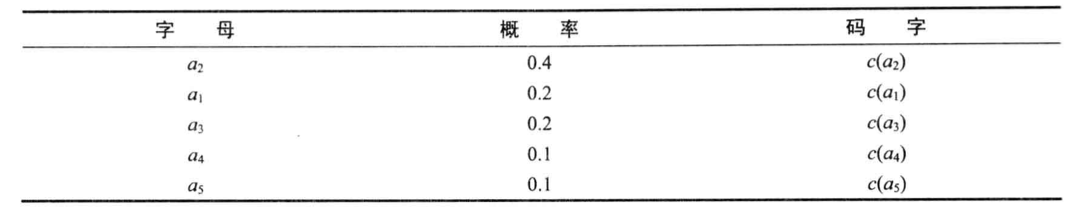
\includegraphics[scale=0.7]{/Users/_linxinhui_/Desktop/DSACurriculumDesign/IntroductionToHuffmanCodingAlgorithm/pics/1.png}
\caption{含有五个字符的原符号集}
\end{figure}

概率最低的两个符号为\(a_4\)和\(a_5\), 指定其码字如下:

\begin{gather*}
c(a_4) = \alpha_1 * 0 \\
c(a_5) = \alpha_1 * 1
\end{gather*}

其中\(\alpha_1\)是二进制位串, \(*\)表示拼接。

现在定义一个新的符号集\(A'\), 它包括四个字母: \(a_1, a_2, a_3, a_4'\),
其中\(a_4'\)由\(a_4\)和\(a_5\)组成,
其概率为\(P(a_4') = P(a_4) + P(a_5) = 0.2\), 按概率降序重排符号集:

\begin{figure}[H]
\centering
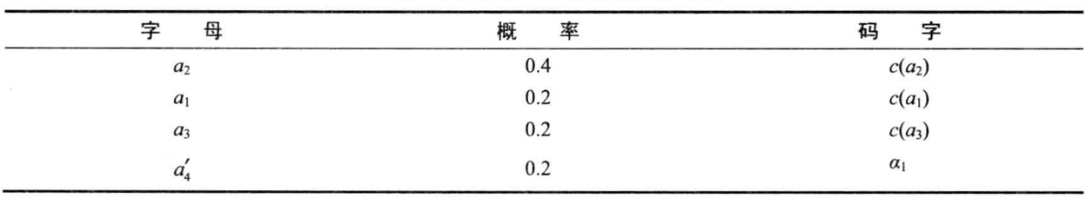
\includegraphics[scale=0.7]{/Users/_linxinhui_/Desktop/DSACurriculumDesign/IntroductionToHuffmanCodingAlgorithm/pics/2.png}
\caption{包含四个字母的缩减符号集}
\end{figure}

在这个符号集中, \(a_3\)和\(a_4'\)是出现概率最低的两个字母,
指定其码字如下:

\begin{gather*}
c(a_3) = \alpha_2 * 0 \\
c(a_4') = \alpha_2 * 1
\end{gather*}

又\(c(a_4') = \alpha_1\), 故有:

\[\alpha_1 = \alpha_2 * 1\]

从而:

\begin{gather*}
c(a_4) = \alpha_2 * 10 \\
c(a_5) = \alpha_2 * 11
\end{gather*}

重复上述过程, 定义包含三个字母\(a_1, a_2, a_3'\)的新符号集\(A''\),
其中\(a_3'\)由\(a_3\)和\(a_4'\)组成,
概率为\(P(a_3') = P(a_3) + P(a_4') = 0.4\), 按概率降序重排符号集:

\begin{figure}[H]
\centering
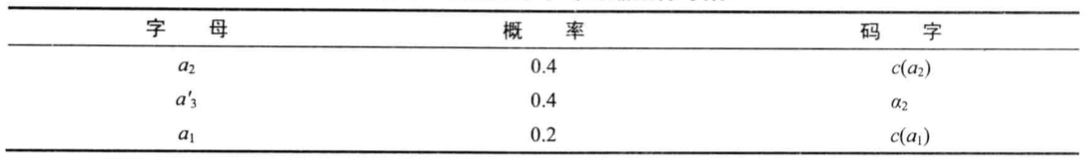
\includegraphics[scale=0.7]{/Users/_linxinhui_/Desktop/DSACurriculumDesign/IntroductionToHuffmanCodingAlgorithm/pics/3.png}
\caption{包含三个字母的缩减符号集}
\end{figure}

出现概率最低的两个符号为\(a_3'\)和\(a_1\), 故:

\begin{gather*}
c(a_3') = \alpha_3 * 0\\
c(a_1) = \alpha_3 * 1
\end{gather*}

又\(c(a_3') = \alpha_2\), 有:

\[\alpha_2 = \alpha_3 * 0\]

从而:

\begin{gather*}
c(a_3) = \alpha_3 * 00 \\
c(a_4) = \alpha_3 * 010 \\
c(a_5) = \alpha_3 * 011
\end{gather*}

继续, 定义包含两个字母\(a_3''\)和\(a_2\)的符号集\(A'''\),
其中\(a_3''\)由字母\(a_3'\)和\(a_4\)组成,
概率为\(P(a_3'') = P(a_3') + P(a_1) = 0.6\), 排序, 得下表:

\begin{figure}[H]
\centering
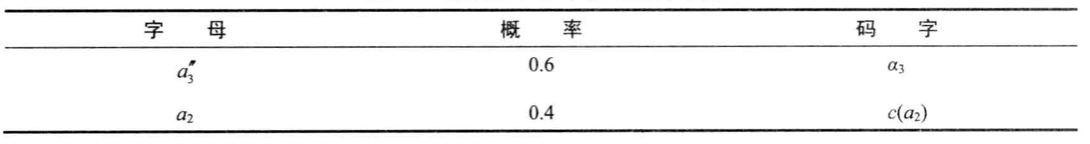
\includegraphics[scale=0.7]{/Users/_linxinhui_/Desktop/DSACurriculumDesign/IntroductionToHuffmanCodingAlgorithm/pics/4.png}
\caption{包含两个字母的缩减符号集}
\end{figure}

只剩下两个字母, 分配码字:

\begin{gather*}
c(a_3'') = 0 \\
c(a_2) = 1
\end{gather*}

这意味着\(a_3 = 0\), 从而:

\begin{gather*}
c(a_1) = 01 \\
c(a_3) = 000 \\
c(a_4) = 0010 \\
c(a_5) = 0011
\end{gather*}

Huffman码生成完毕:

\begin{figure}[H]
\centering
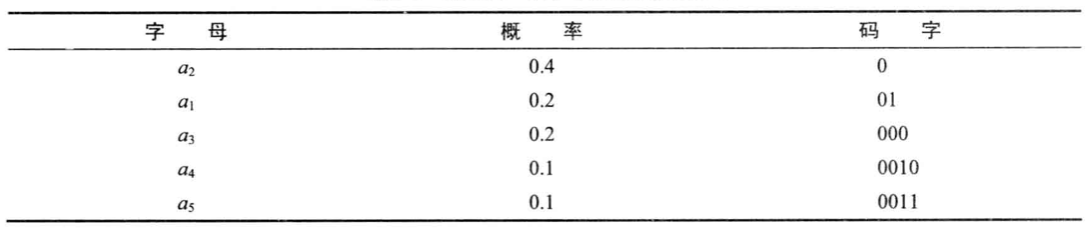
\includegraphics[scale=0.7]{/Users/_linxinhui_/Desktop/DSACurriculumDesign/IntroductionToHuffmanCodingAlgorithm/pics/5.png}
\caption{原五字母符号集的Huffman码}
\end{figure}

编码过程示意如下:

\begin{figure}[H]
\centering
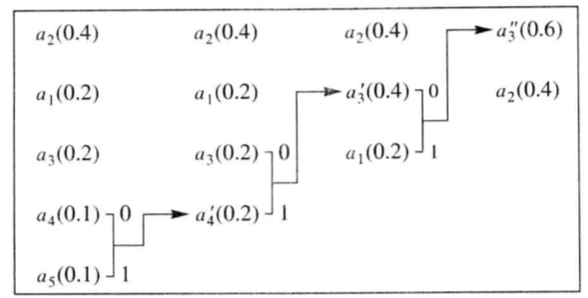
\includegraphics{/Users/_linxinhui_/Desktop/DSACurriculumDesign/IntroductionToHuffmanCodingAlgorithm/pics/6.png}
\caption{编码过程, 括号里是符号出现的概率}
\end{figure}

Huffman码是一种前缀码, 因此可以将其表示为二叉树, 树中的叶节点与符号对应,
由此可以得到另外一种构造Huffman码的方法:

从叶节点开始构造Huffman树。由于概率最小的两个符号的码字除最后1比特外都相同,
故在从根节点遍历到与这两个符号对应的叶节点时,
除最后一步之外的所有路径都相同。由此又可以推出,
这两个最低概率符号对应的叶节点是同一节点的子节点。我们将最低概率符号的相应叶节点连接到同一个节点,
然后将这个节点看做缩减符号集中的一个符号。这个符号的概率等于其子节点概率之和。接着对缩减符号集的对应节点进行排序,
在这个缩减符号集中找出概率最小的两个符号,
并继续用上述规则为相应节点生成一个父节点。如此继续知道只剩下一个节点,
也就是根节点, 如此构造出Huffman树, 要得到每个符号的代码,
从根节点遍历到每个叶节点, 为左分支指定0,
为右分支指定1即可得到Huffman码。

反之, 给定Huffman树和一个位串, 解码的过程如下:
从根节点遍历到与某符号对应的叶节点, 就可以得到该节点的代码,
遍历路径上的每条分支都向码字贡献一个比特的数据(每条左分支贡献一个0,
每条右分支贡献一个1)。反之, 当知道码字时,
每次译码(一次翻译一个字符)都从根节点开始, 遇到\texttt{0}走左分支,
遇到\texttt{1}走右分支, 直到走到叶子节点, 重复该过程直到码字全部被译出。

以上构造Huffman码的算法是相对自然的(便于区分,
我们不妨称之为朴素Huffman码或一般性Huffman码),
尽管生成的Huffman已经是最优前缀码,
根据具体应用场景的不同还可以稍作修改优化。

(对于Huffman码的最优性, 在这里只给出结论而不作证明。)

\subsubsection{最小方差Huffman码(Minimum Variance Huffman Code)}\label{header-n492}

对上述算法稍作修改, 将合并产生的新字母尽可能放在列表中较高的位置以减小码字长度的方差。

我们在排序时, 尽可能将合并的新字母放到列表中最高的位置, 具体地说即是: 列表按出现频率降序排列, 假设\(a\)是原字符集中的字母, \(a'\)是所谓合并字符, 且\(P(a') = P(a)\), 则在列表中\(a'\)的位置在\(a\)之上。

承上例, 借助二叉树展示最小方差Huffman码的生成过程:

\begin{figure}[H]
\centering
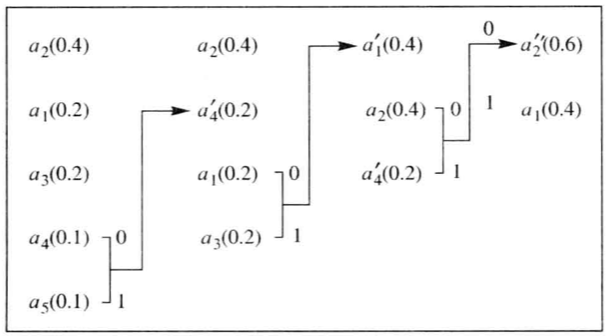
\includegraphics{/Users/_linxinhui_/Desktop/DSACurriculumDesign/IntroductionToHuffmanCodingAlgorithm/pics/7.png}
\caption{最小方差Huffman码的生成过程}
\end{figure}

生成的Huffman码如下:

\begin{figure}[H]
\centering
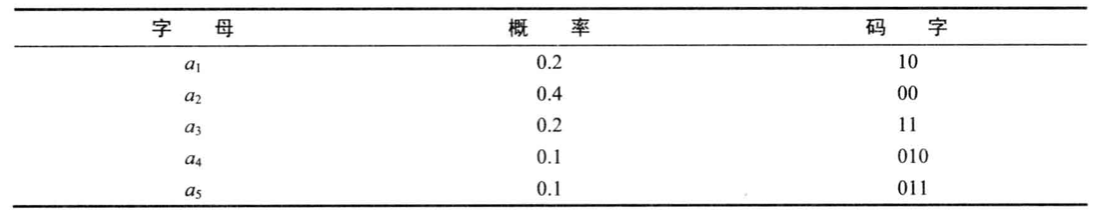
\includegraphics[scale=0.7]{/Users/_linxinhui_/Desktop/DSACurriculumDesign/IntroductionToHuffmanCodingAlgorithm/pics/8.png}
\caption{最小方差Huffman码}
\end{figure}

以下内容引自 \emph{Introduction to Data Compress} :

\begin{quote}
请记住, 在许多应用中, 尽管正在使用的可能是变长代码, 但可供使用的传送速度通常是固定的。例如, 如果要以10000符号/秒的速度传送上述符号集中的符号, 那就要求传输容量为22000比特/秒。这意味着在每一秒内, 预计信道会不多不少正好接收22000比特。由于比特生成速率会在22000比特/秒上下变化, 所以信源编码器的输出一般会被放入一个缓冲区。缓冲区的目的是平滑比特生成速率的变化。但是, 缓冲区的大小是有限的, 码字中的方差越大, 缓冲区设计问题就变得越困难......
\end{quote}

总而言之, 使用最小方差Huffman码能够有效地减少编码赤字(信源发送信息的比特数和信道期望接受比特数的差值), 在编码冗余度相同不变的情况下简化编码器缓冲区的设计, 因此在实际通信系统的设计中更为合理。

\subsubsection{范式Huffman码(Canonical Huffman Code)}\label{header-n503}

Huffman码是一种最优的前缀编码技术, 然而其存在的不足却制约了它的直接应用。其中最为重要的是, 解码器需要知道Huffman编码树的结构, 因而编码器必须为解码器保存或传输Huffman编码树。对于小量数据的压缩而言, 这是很大的开销。因而, 应用Huffman码的关键是降低Huffman编码树占用的存储空间。

降低Huffman编码树的存储空间的手法包括但不限于以下几种:

\begin{enumerate}
\def\labelenumi{\arabic{enumi}.}
\item
  自适应Huffman编码技术
\item
  使编码器和解码器使用事先约定的编码树
\item
  使用所谓范式Huffman码
\end{enumerate}

自适应Huffman编码技术即在使用某种约定的条件下, 解码器能动态地重构出和编码器同步的Huffman编码树而不需要任何附加数据, 这样做能使Huffman编码树的存储空间降为零, 而代价是时间开销的增大。

而所谓使编码器和解码器使用事先约定的编码树这种方法只能针对特定数据使用, 不具备通用性。

最为常用的方法是范式Huffman码。

范式Huffman码可以看做一般Huffman码的一个子集。其原理是: 使用某些强制的约定, 仅通过很少的数据便能重构出Huffman编码树的结构。其中一种很重要的约定是数字序列属性(numerical sequence property), 它要求:

\begin{enumerate}
\def\labelenumi{\arabic{enumi}.}
\item
  相同长度的码字是连续整数的二进制描述。例如, 假设码字长度为4的最小值为0010(所谓最小值指的是按从小到大的顺序排列所有4位二进制串中不产生悬挂后缀的最小值, 具体取决于码字长度小于4的编码), 那么其它长度为4的码字必为0011, 0100, 0101, ...
\item
  为了尽可能的利用编码空间, 长度为\(i\)第一个码字\(f(i)\)必须能从长度为\(i-1\)的最后一个码字得出, 即: \(f(i) = 2(f(i-1)+1)\)。假定长度为4的最后一个码字为1001, 那么长度为5的第一个码字便为10100
\item
  码字长度最小的第一个编码从0开始
\end{enumerate}

通过上述约定, 解码器能根据每个码字的长度恢复出整棵Huffman编码树的结构。

综上, 范式Huffman是一种能够高效存储的Huffman码, 只需要对长度列表进行编码即可(解码时重构树, 摆脱了对树的依赖), 极大地节省了编码译码的空间成本, 范式Huffman码的应用场景很广泛, GZIB、ZLIB、PNG、JPEG、MPEG等压缩方法都是用了范式Huffman码。

\subsubsection{有限长度Huffman码(Finite Length Huffman Code)}\label{header-n526}

Huffman算法的目的在于降低码字的平均长度, 但并没有限制单个码字的最大长度。设想符号集极大的情形,
可能出现非常长的Huffman编码, 其结果是码字可能无法放入单个机器字(也即其长度超过了机器字长), 同时也会降低编码效率。

\begin{quote}
机器字长是指计算机进行一次整数运算所能处理的二进制数据的位数
\end{quote}

为了避免上述问题, 我们在设计变长编码的过程中增加一个约束条件, 即要求所有码字不大于某一长度\(l_{max}\)。

构造有限长度Huffman码的算法需要用到\texttt{Kraft-McMillan不等式}和\texttt{打包-合并算法}(该算法是应用最广泛的用于构造有限长度Huffman码的算法, 注意它的用途包括但不限于构造Huffman码), 具体过程比较复杂, 而有限长度Huffman码依然不是现在需要关心的内容, 从略。

\subsection{非二进制Huffman码(Non-binary Huffman Code)}\label{header-n532}

将二进制Huffman码推广到非二进制Huffman码的思路十分简单, 其条件是代码元素来自m元符号集, 其中m大于等于3。仿照二进制Huffman生成的过程, 非二进制Huffman码有以下特点:

\begin{enumerate}
\def\labelenumi{\arabic{enumi}.}
\item
  高频符号的码字短于低频符号
\item
  出现频率最低的m个符号具有相同码长
\item
  概率最低的m个符号仅最后一位不同
\end{enumerate}

设想有一个包含6个字母的信源, 为它设计一种三元Huffman码。在缩减符号集的过程中既有取两个字符合成一个新字符的操作, 又有取三个字符合成一个新字符的操作, 由此导致了不同的生成Huffman的方案。

遇到这样的情况, 注意到概率最小的符号将拥有最长的码字, 且所有被合并为一个复合符号的符号都具有相同长度的码字。这意味着我们在第一阶段(也即第一步, 下同)合并的所有字母都具有相同长度的码字, 这些码字是所有码字中最长的。如果在某一阶段, 允许合并不足m个符号, 那最适合的时机正是第一阶段。

一般地, 在代码有\(m\)元, 符号集中有\(M\)个字母情况下, 设第一个阶段应当合并\(m'\)个字母, 则\(m'\)满足:

\begin{enumerate}
\def\labelenumi{\arabic{enumi}.}
\item
  介于\(2\)与\(m\)之间
\item
  使得 \(m'mod(m-1) = Mmod(m-1)\)
\end{enumerate}

具体的使用非二进制Huffman码的例子这里不给了, 展示一棵非二进制Huffman编码树, 显然非二进制Huffman码的编码树不再是二叉树(事实上也未必是m叉树):

\begin{figure}[H]
\centering
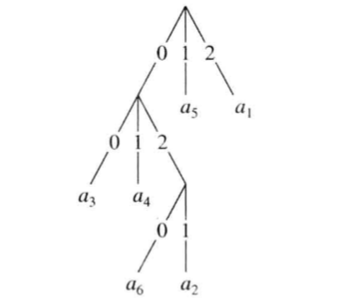
\includegraphics{/Users/_linxinhui_/Desktop/DSACurriculumDesign/IntroductionToHuffmanCodingAlgorithm/pics/9.png}
\caption{非二进制Huffman码的编码树}
\end{figure}

\subsection{自适应Huffman码(Adaptive Huffman Code)}\label{header-n551}
\subsubsection{自适应Huffman码相比朴素Huffman码(Adaptive Huffman Code vs. Simple Huffman Code)}\label{header-n552}

朴素的Huffman算法给出了一种静态的编码树构造方案, 在编码前需要收集统计信息, 而后才能开始编码, 也即在编码是需要进行两遍扫描, 然而第一次扫描一方面需要时间和空间成本, 另一方面在某些情境下是难以实现的(比如大多数多媒体应用场景)。

除此之外, 静态编码树构造方案不能对符号流的局部统计规律变化做出反应, 因为它从始至终都使用完全不变的编码树。而自适应Huffman编码不需要事先构造Huffman树, 而是随着编码的进行逐步构造Huffman树。同时, 这套编码系统对符号的统计也动态进行, 随着程序的运行, 同一个符号的编码可能发生改变。

最后, 静态编码在储存或传输Huffman编码结果之前, 还必须先储存或传输Huffman编码树, 自适应霍夫曼编码则不需要, 这大大节省了内存开销。

综上, 自适应Huffman码相比于朴素Huffman码有诸多好处, 这里简单介绍Huffman的原理和构造过程(至于实现......依然不是目前的重点, 留待有缘再见)。

\subsubsection{自适应Huffman码的构造(Create Adaptive Huffman Code)}\label{header-n557}

向Huffman树节点增加两个属性:\texttt{(节点)权重}和\texttt{(节点)编号}。并规定同一父节点的后代称为兄弟(sibling)。

其中, 叶子节点的权重指该节点对应字符出现的次数, 内部节点的权重则是其后代权重之和。

对自适应哈夫曼树满足, 有如下两个原则:

\begin{enumerate}
\def\labelenumi{\arabic{enumi}.}
\item
  父节点的节点编号一定比子节点大
\item
  节点编号大的节点, 权重值也一定大
\end{enumerate}

这两个原则被称为兄弟属性, 任何具有兄弟属性的树都是Huffman树, 而构造自适应Huffman码的过程就是在编码过程中实时调整哈夫曼树以保证满足兄弟属性, 其过程简单描述如下:

\begin{enumerate}
\def\labelenumi{\arabic{enumi}.}
\item
  建立只有一个节点(根节点)的Huffman树, 根节点标识为NYT(Not Yet Transmitted)
\item
  读取一个字符, 当这个字符没有在哈夫曼树里出现过的时候, 构建新子树, 根节点权重值为1, 左孩子为NYT,右孩子为该字符, 用子树替换上一步标识为NYT的节点。同时输出NYT的编码和字符。当字符出现过时, 输出该字符的哈夫曼编码
\item
  从被输出的节点开始往上走, 每一个节点权重值加1, 但是在加权重值之前, 需要判断该节点是否为同权重值里节点编号最大的。如果不是为最大, 则与最大节点交换位置(节点的子树也要交换而不是只交换单个节点)。交换后再互换节点编号, 这样权重值需要被加1的节点就保证为同级节点编号最大的节点。
\end{enumerate}

\subsection{Huffman码的外延(Extension of Huffman Code)}\label{header-n574}

\begin{quote}
霍夫曼编码算法是最著名的变长编码算法之一, 但还有其他一些知名度较低的算法, 在特定条件下可能非常有用。具体来说, Golomb-Rice码和Tunstall码正在变得越来越流行。
\end{quote}

Golomb-Rice码和Tunstall码在某些方面与Huffman码的设计方法类似, 这里尽可能简单地介绍几句:

\begin{enumerate}
\def\labelenumi{\arabic{enumi}.}
\item
  Golomb码

  \begin{quote}
  Golomb编码是一种无损的数据压缩方法, 由数学家Solomon W.Golomb在1960年代发明。Golomb编码只能对非负整数编码, 符号表中的符号出现的概率符合几何分布(Geometric Distribution)时, 使用Golomb编码可以取得最优效果, 也就是说Golomb编码比较适合小的数字比大的数字出现概率比较高的编码。它使用较短的码长编码较小的数字, 较长的码长编码较大的数字。
  \end{quote}
\item
  Rice码

\begin{quote}
Rice码由数学家Robert F. Rice, 是以哥伦布编码为基础做改良而更简易的前缀码。Rice码可视为适应性编码的一种或是哥伦布编码的特例之一。哥伦布编码有一个可调整参数, 可以是任一正整数。而Rice编码则是此调整参数为2的次方情况时。这让Rice编码在电脑运算上快速许多,  因为计算机上的运算几乎完全基于二进制。Rice编码是一种熵编码技术, 可用在影像及图像压缩上。
\end{quote}
\item
Tunstall码
\end{enumerate}

\begin{quote}
之前讨论的所有编码体系, 在对信源符号集中的字母进行编码时, 都使用不同比特数的码字: 比特数较少的码字用于高频码字, 比特数较多的码字用于低频码字。Tunstall码是一重要的例外。在Tunstall码中, 所有码字的长度相等。但是, 每个码字表示不同数量的字母。
\end{quote}

举个例子, 符号集 \(A = \{A, B\}\) 的2位Tunstall码如下:

\begin{figure}[H]
\centering
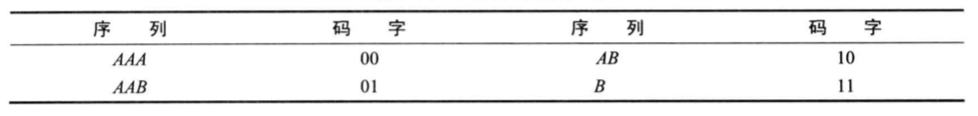
\includegraphics[scale=0.7]{/Users/_linxinhui_/Desktop/DSACurriculumDesign/IntroductionToHuffmanCodingAlgorithm/pics/Tunstall.png}
\caption{Tunstall码的例子}
\end{figure}

\begin{quote}
使用Tunstall码的最大的好处是码字中的误差不会传播, 这一点与其他变长码不同, 比如在Huffamn码中, 一个码字中的错误会导致一系列错误。
\end{quote}

\section{Huffman编码的实现(Implementation of Huffman Coding)}\label{header-n595}

这里的实现指的是朴素Huffman算法/编码的实现, 是课程设计的另一个部分, 也即所谓的Huffman\_En-Decoder。

这个编解码器的设计、具体代码实现以及运行结果截图见对应的文件夹, 这里不再赘述了。

\end{CJK}
\end{document}